\chapter{Introduction} \label{chap:intro}

The purpose of this chapter is to introduce the motivation for the work, briefly describe the problem at hand and outline the work that will be developed, as well as the structure of the thesis.

\section{Motivation} \label{sec:motivation}

Collective software development requires the handling of merge conflicts, as conflicts between parallel work arise. Called merge conflicts, as they arise when this parallel work is merged, they vary in their difficulty of detection.
Common textual conflicts, where the same line is altered by multiple people, are automatically detected by version control systems, allowing amendments to be easily made. However not all conflicts are so easily detected and their occurence can bring with it the addition of software bugs to the system. Semantic merge conflicts, in particular, are hard to detect, both by software and human review and remain a hard to solve situation. Given that around 30\% of developers do not even actively monitor for merge conflicts and of those who do, mostly do it with reactive strategies~\cite{kn:lifecycle}, the ability to automatically detect these would be a great boon for the field of software development, especially as by developers own admissions, the longer a merge conflict is left unsolved, the harder it becomes to resolve it: ``Untangling takes days instead of minutes when it gets too out of hand.''~\cite{kn:lifecycle}.

The recent revolution in the field of Large Language Models (LLMs) may prove to add a valuable tool in tackling this, given their ability to describe the functioning of code snippets as well as generate them. These capabalities may allow us, with the correct development and prompting, to not only describe the semantic conflict present in a specific merge commit, but also to generate the appropriate unit test that identifies the lost or emergent behaviour associated with it.


\section{Problem} \label{sec:problem}

To manage the concurrent work of several developers in software projects, it is common to employ \emph{version control systems} (hereby referred as \emph{VCS}), which can be defined as ``a system that manages the development of an evolving object. In other words, it is a system that records any changes made by the software developers.''~\cite{kn:vers_review}.

A significant task of version control is managing access to shared resources.
With ``pessimistic locking'' a lock-modify-unlock paradigm was adopted, where a given file would be locked for modification while it is being modified, thus ensuring each resource can only be handled by one actor at a time. VCS's however, generally implement a copy-modify-merge mechanism: concurrent work can done on a resource, with joining the parallel work together handled by merges afterwards, with two ``branches'' of work merged into one~\cite{kn:vers_ott}.

Merge conflicts arise when parallel work cannot be automatically merged. Of this, several different types exist, as summarized by \citet{kn:tmens}:

Textual conflicts occur when the same textual elements of code are modified in both branches of a merge. For example, when the same line of code is modified by two people in their respective branches.

Syntactic conflicts arise from parallel changes that when merged do not generate textual conflicts, but the resulting merge creates code that is invalid given the languages rules. For example, programmer A renames a variable, while programmer B uses the variable somewhere (with the original name). There is no textual conflict, but the code will not compile due to the usage of an uninitialized variable.

Finally semantic conflicts occur when parallel changes do not have any textual conflict and their merge is syntactically valid, but the resulting code does not behave as expected, or exhibits lost or new unexpected behaviour.

Most VCS's, such as Git, implement textual merge tools (ergo, they can only identify textual conflicts). However there are specialized tools that handle other types of merges. for instance Turbomixer is also able to handle syntactic merges~\cite{kn:tmens}. The focus on textual merging is unsurprising as around 90\% of conflicts are textual~\cite{kn:lcsd} and syntactic conflicts are easy to identify after merging, as errors will be clearly indicated and programs will not compile.
Semantic conflicts remain as both undetected by VCS's and hard to detect after merges. Thus, finding methods to automatically identify and highlight semantic conflicts in merge commits has been a persistent problem and a source of study in the field~\cite{kn:nuno,kn:leuson,kn:leuson2}.

As a simple example of a merge conflict, consider a class ``Cart'' of a shopping app, subject to concurrent changes in two branches, as shown in \Cref{fig:conflict}.
Initially Cart just has a method total\_cost that calculates the total cost given a percentage of discount.
In branch A the existing method is modified to take both tax and discount as parameters and the method is overloaded by a new version that only takes the tax parameter.
In branch B, a checkout method is added, which calls the original total\_cost method. After merging, no error appears, but the checkout function will be running the total\_cost tax method, expecting the calculation of a discount. The example is shown in \Cref{fig:conflict}.

From here the conflict arises, as after merging the behaviour of the checkout function is not the intended one: instead of calculating the cost with a discount, it now uses the value given for discount as a tax.
To identify this conflict, we would need to generate a test that would find evidence of this emergent behaviour: in this case with a test for checkout that calculates the expected cost with tax. This test would pass on the merge commit and fail in Branch B and not compile in A (as checkout is not introduced),
certifying that due to the semantic conflict, new unexpected behaviour has been introduced.

\begin{figure}[t]
    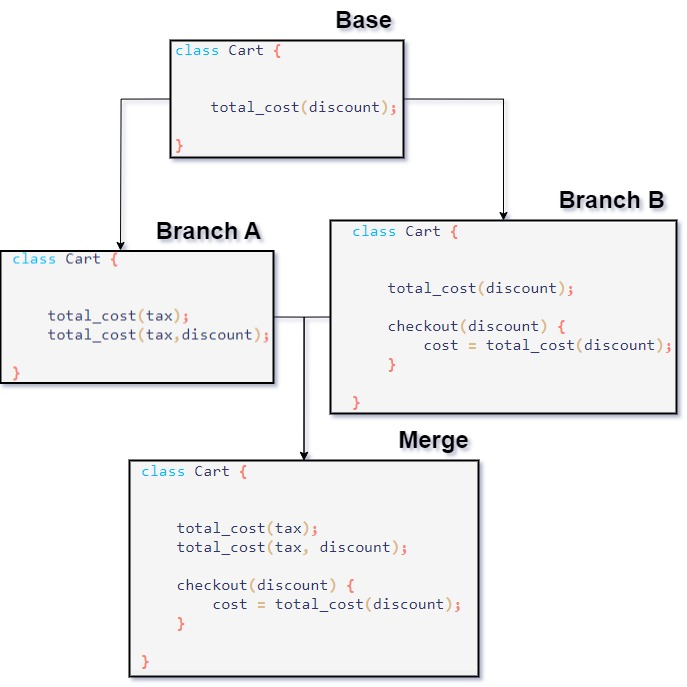
\includegraphics[width=0.86\textwidth]{conflict}
    \caption{Model of the motivating example conflict, with Base, Branch A, Branch B and Merge versions of the code.}
    \label{fig:conflict}
\end{figure}

\section{Goal} \label{sec:goal}

The goal of this research project is to assess to what extent existing Large Language Models can be used to identify semantic conflicts, both textually and through the generation
of appropriate unit tests. By comparing our results to existing prompts for unit test generation, we will assess to what extent, if any, we improved on and how to further develop
unit test generation for semantic conflicts using LLMs, hopefully opening avenues for fully automated systems that identify and alert developers to this type of conflict.

\section{Study} \label{sec:study}

Following an initial exploratory phase, where different prompts, techniques and models were experimented with, our work approaches the issue by answering
3 research questions:

\begin{itemize}
    \item[\textbf{RQ1:}] Can ChatGPT identify the presence of a semantic conflict, as well as explain it?
  
    \item[\textbf{RQ2:}] Given an explanation of a semantic conflict in a merge
    commit, can ChatGPT generate unit test case that are able to identify it?
  
    \item[\textbf{RQ3:}] Can state-of-the-art prompts lead ChatGPT to generate to
    unit test cases that are able to identify semantic conflicts?  How do their
    results compare to the results of the prompt used in RQ2?
  \end{itemize}

\section{Thesis Structure} \label{sec:struct}


\Cref{chap:intro} introduces the topic and problem at hand.
\Cref{chap:rw} details existing related work on the topics at hand.
\Cref{chap:study} described our study and research questions and \Cref{chap:results} answers each research question.
\Cref{chap:conclusion} gives a conclusion.
